% !TEX root = Main document.tex
\section{Experimental method}

\subsection{Experimental setup}
All experiments were performed in the Twente Turbulent Taylor-Couette (T$^3$C) facility described in~\citet{VanGils2011} and shown in figure~\ref{fig:T3C}.
 It consists of two independently rotating concentric cylinders of length $L = \SI{0.927}{\metre}$. The inner cylinder is fabricated from grade 316 hydrophilic stainless steel. The outer cylinder is cast from clear acrylic, which allows for full optical access to the flow between the cylinders. The inner radius of the outer cylinder is $r_o = \SI{0.279}{\metre}$ %0.2794
and the outer radius of the inner cylinder equals $r_i~=~\SI{0.200}{\metre}$, thus the radius ratio is $\eta = r_i / r_o = 0.716$. %0.7158
 The resulting gap has a width $d = r_o - r_i =
\SI{0.079}{\metre}$
 and was filled with \add{fully air saturated deionized} water. For inner cylinder rotation, the Reynolds defined, based on the gap width and velocity of the inner cylinder is
\begin{equation}\label{eq:Rey}
\Rey = \frac{\omega_i r_i d}{\nu},
\end{equation}
where $\omega_i$ is the angular velocity of the inner cylinder and $\nu$ is the kinematic viscosity of the working fluids. The inner cylinder rotates at frequencies in the range $\omega_i = \SIrange{5}{18}{\hertz}$, while the outer cylinder is kept stationary. Typical values used in this research range from $\Rey = 5 \times 10^5$ to $\Rey = 1.8 \times 10^6$. The system is actively cooled to keep the temperature of the working fluid at $\SI{21}{\degreeCelsius} \pm \SI{0.5}{\degreeCelsius}$.

\begin{figure}
    \centering
   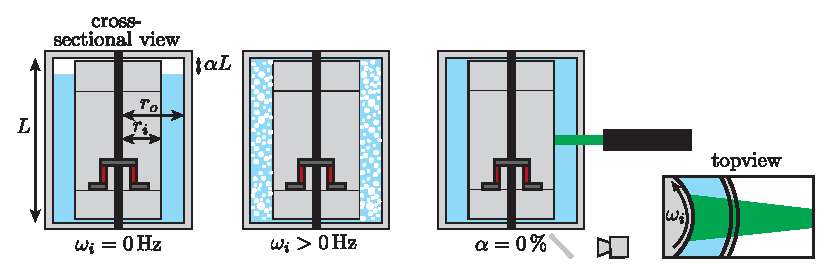
\includegraphics{Figures/fig1}
    \caption{Schematic overview of the measurement setup. Shown are the outer and inner cylinder, of which the latter consists of three sections. The middle section is connected to the driving shaft by means of a torque sensor, which is also shown in the figure. The gap between the two cylinders $r_o - r_i$ is filled with water and air, of which the quantity of the air is expressed by means of a void fraction $\alpha$, ranging between \SI{0}{\percent} and \SI{6}{\percent}. When the inner cylinder is rotating ($\omega_i > \SI{0}{\hertz})$, bubbles are formed and distributed in radial and axial direction over the gap due to turbulent mixing. Particle Image Velocimetry (PIV) measurements can be done only when there are no bubbles present in the working liquid ($\alpha = \SI{0}{\percent}$). The PIV lasersheet is placed at cylinder mid-height and the flow is observed through a window in the bottom-plate using a mirror and a camera.}\label{fig:T3C}
\end{figure}

By partly filling the apparatus, as in figure~\ref{fig:T3C}, we vary the volume fraction of air $\alpha$ in the working fluid from \SI{0}{\percent}~to~\SI{~6}{\percent}. The turbulence mixes the air and water, generating bubbles that are distributed over the height and over the gap between cylinders~\citep{vanGils2013}.

\subsection{Torque measurements}
The inner cylinder is composed of three sections. The torque exerted by the fluid on the inner cylinder is measured using a Honeywell 2404-1K hollow reaction torque sensor that is placed inside the middle section of the inner cylinder as indicated in figure~\ref{fig:T3C}. Only the torque on the middle section of length $L_{\text{mid}} = 0.536$~m is taken into account to reduce end-plate effects between the rotating lid of the inner cylinder and the stationary lid of the outer cylinder. We express the torque in non-dimensional form using the skin friction coefficient:
\begin{equation}\label{eq:cf}
C_f = \frac{\mathcal{T}}{L_{\text{mid}}\rho\nu^2\Rey^2}
\end{equation}
where $\mathcal{T}$ denotes the torque, $\rho$ and $\nu$ are the density and kinematic viscosity, respectively, of the working fluid. \\
The drag reduction for the {hydrophobic} coating and the hydrophilic reference is determined using equation~(\ref{eq:DR1}).
\begin{equation}\label{eq:DR1}
\text{DR}(\alpha) = 1 - \frac{C_{f}(\alpha)} {C_{f}(\alpha=0)}
\end{equation}
This shows the influence of adding bubbles to the flow on the drag. The difference in drag reduction $\Delta\text{DR}$ between a {hydrophobic} inner cylinder (IC) and a hydrophilic IC is defined as
\begin{equation}\label{eq:deltaDR}
\Delta\text{DR}(\alpha) = DR_\text{hydrophobic}(\alpha) - DR_\text{hydrophilic}(\alpha)
\end{equation}
In order to provide insight into the influence of the {hydrophobic} IC on the flow, we define a {\it net} drag reduction as
\begin{equation}\label{eq:DR2}
\text{DR}_\text{\it net}(\alpha) = 1 - \frac{C_{f,\text{hydrophobic}}(\alpha)}{C_{f,\text{hydrophilic}}(\alpha = 0)}
\end{equation}
Here $C_{f,\text{hydrophobic}}(\alpha)$ is the skin friction coefficient for the {hydrophobic} IC and different values of $\alpha$, and $C_{f,\text{hydrophilic}}(\alpha = 0)$ is the skin friction coefficient for the smooth hydrophillic inner cylinder, without air bubbles present in the flow ($\alpha$ = 0). In equation~(\ref{eq:DR1}) the focus is only on the influence of bubbles on the drag, with either a {hydrophobic} or a hydrophilic IC, whereas equation~(\ref{eq:DR2}) show the influence of both drag reducing measures: bubbles and a {hydrophobic} coating.

\subsection{{hydrophobic} coating}
In the {hydrophobic} case, the IC of the T$^3$C is fully coated with a 3M~Membrana Accurel\textsuperscript{\textregistered}~PP~2E~HF flatsheet membrane. This porous hydrophobic polypropylene material is commercially available in the large quantities that are needed to cover the complete IC.
This coating is supplied on rolls that have a width of about \SI{27}{\cm}. It is attached to the inner cylinder using double-sided adhesive tape. From visual inspection it is estimated that \SI{99}{\percent} of the IC is covered by the coating, see figure~\ref{fig:photo_coating_glow}.

We used a Dataphysics OCA 15EC device to measure the contact angle hysteresis for both the {hydrophobic} coating and the reference case, which is the hydrophilic, uncoated steel IC. The {hydrophobic} coating has advancing and receding water contact angles of $\SI{152}{\degree} \pm \SI{2}{\degree}$ and $\SI{120}{\degree} \pm \SI{5}{\degree}$, respectively. For the hydrophilic IC, an advancing contact angle of $\SI{93}{\degree} \pm \SI{2}{\degree}$ was found. The receding contact angle is set at \SI{10}{\degree}, which is the lowest angle the setup could measure.

\begin{figure}
\centering
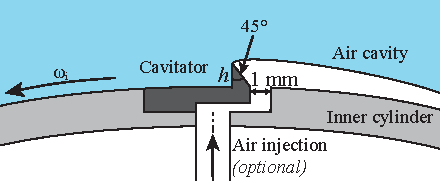
\includegraphics[width=\textwidth]{Figures/fig2}
\caption{SEM photos of the side of the coating that is exposed to the flow. The top row focuses on a region composed of smaller pores. The bottom row shows a region with larger pores.}\label{fig:SEM-bottom}
\end{figure}

\subsection{Roughness}
The machining process to fabricate the standard hydrophilic IC gives a surface roughness of $k_{ic} = \SI{1.6}{\um}$. The viscous length scale $\delta_\nu$ is derived from the measured torque data, as discussed in~\citep{hui13}. For the maximum Reynolds number $\Rey_\text{max} = 1.8 \times 10^6$ used in this research, the viscous length scale reaches its lowest value of $\delta_\nu = \SI{1.9}{\um}$. The resulting roughness in wall units $k^+_{ic} \approx 0.8$. Therefore, the uncoated hydrophilic IC can be assumed to be a hydrodynamically smooth surface.

The average roughness of the coating is analysed from its pore size using 24 different SEM images, made using three different magnifications, as shown in figure~\ref{fig:SEM-bottom}. \add{The coating consists of an isotropic sponge-like structure, meaning that the cross section looks similar to the top and bottom surface. Therefore we use SEM images of the top surface to evaluate the size and roughness of the pores.} The SEM images show a distribution of pore sizes, in the range of \SIrange{1}{10}{\um}. The pores that correspond to the smaller length scale are found in regions separated by pores of the larger length scale. The size distribution is quantified with the image processing program ImageJ, using edge detection of the thresholded image (Analyse Particles tool). Eight different images of the smallest magnification were used for this. The images were pre-processed by subtracting a sliding background and by applying a local mean threshold algorithm. Eroding and dilation was used to remove small scale noise. It is difficult to define the error for the pore size distribution, since it is difficult to evaluate the edge of a pore from the perspective of the flow. For instance in figure~\ref{fig:SEM-bottom}, when inspecting the large pores at highest magnification, we see thin thread-like fibres that span across a pore. Whereas in the image analysis this might be detected as an edge, the flow might experience this differently. However, from the SEM images and the pore size distribution it is clear that multiple roughness length scales are present on the surface of the coating. Hence, dependent of $\Rey$, a larger or smaller fraction of the surface plays a role in influencing the flow. The resulting distribution of binned pore sizes is shown in figure~\ref{fig:poresize_plot}. The combined area of all pores with diameter $D_p$ over the total area, the fraction $A/A_0$, is plotted versus $D_p$. A maximum is found at $D_p = \SI{2.5}{\um}$, although the larger length scales that are more relevant to the flow are also found.


\begin{figure}
\centering
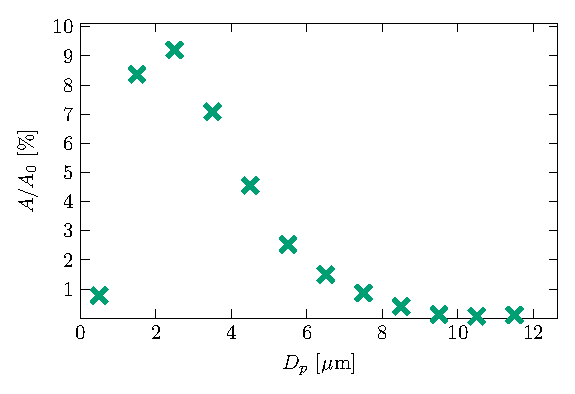
\includegraphics{Figures/fig3}
\caption{Pore size diameter $D_p$ (roughness) distribution of the coating as fraction of coverage $A$ of total area of the coating $A_0$. A range of length scales is observed, corresponding to the different regions identified in figure~\ref{fig:SEM-bottom}. The equivalent circle diameter has been used as a measure of the size $D_p = 2 \sqrt{A_p/\pi}$.} \label{fig:poresize_plot}
\end{figure}

\subsection{Experimental procedure}
During a measurement period of one hour, the IC was accelerated in steps from \SI{5}{\hertz} to \SI{18}{\hertz}, corresponding to a range of $\Rey$ between $5\times10^5$ and $1.8\times10^6$, while continuously measuring torque exerted by the fluid on the inner cylinder.
Every variation of a {hydrophobic} IC with $\alpha > \SI{0}{\%}$ was measured four times. Between changing the volume percent of air $\alpha$, the reference case of $\alpha = \SI{0}{\%}$ air is measured twice, to account for changes to the coating caused by the flow itself. An overview of the measurements is shown in order of execution in table~\ref{table:measurement_order}.
\begin{table}
\centering
\begin{tabular}{ | l | l | l | c | }
\cline{1-4}  \\[-0.9em]
 Surface & $\alpha$ [\%]  & $\omega_i$ [Hz] & Measurements \\ \cline{1-4} \\[-0.9em]
hydrophobic &  0  & 	\numrange{5}{18} & 2 \\
					  &  2 	&  	5--18 & 4 \\
					  &  0 	& 		5--18 & 2 \\
					  &  4 	& 		5--18 & 4 \\
					  &  0 	& 		5--18 & 2 \\
					  &  6 	& 		5--14 & 4\\
					  &  0 	& 		5--18 & 2 \\
\cline{1-4} \\[-0.9em]
hydrophilic   & 0 	& 		5--18 & 2 \\
					  & 2 	& 		5--18 & 3\\
					  & 4 	& 		5--13.4 & 3\\
  					  & 4 	& 		15.8--18  & 3\\
					  & 6 	& 		5--14 & 3 \\ \cline{1-4}

\end{tabular}\caption{Overview of the measurement parameter space, in order of execution. Between changing the volume percentage of air $\alpha$, the reference case of $\alpha = \SI{0}{\%}$ air was measured twice, to account for changes to the coating caused by the flow itself. Deviations from the standard frequency range $\omega_i = \SIrange{5}{18}{\hertz}$ were the result of heavy vibrations in the system, forcing us to skip a certain frequency range.} \label{table:measurement_order}
\end{table}

\subsection{Flow visualisation}
A Nikon D800E camera was used to capture still images of the flow. This provides insight on the presence of an air plastron: air captured by the coating is visible in the form of a silvery reflection on the surface \citet{Shirtcliffe2006,McHale2009,Daniello2009,Poetes2010,Mchale2011,Dong2013,Park2014,Park2015,
Saranadhi2016}. This can be seen in figure~\ref{fig:photo_coating_glow}, where the highlighted area points out locations where the incident light is of the right angle to see the plastron. It was found that an air plastron was present during the measurements featuring a {hydrophobic} IC.
\add{To test the stability of the plastron and force the surface in a wetted state, the surface tension was lowered by adding TritonX surfactant whilst rotating the inner cylinder at $\Rey = 1.0\e{6}$ with single phase flow conditions. From image analysis it was determined that only after \SI{1.5e-4}{\mol \per \litre} TritonX was added, the silvery reflection had completely dissapeared. At this concentration of TritonX the surface tension is about \SI{35}{\milli \newton \per \metre}~\citep{Gobel1997}. So both surface tension and Laplace pressure are about half the value of that for pure water.}

\begin{figure}
\centering
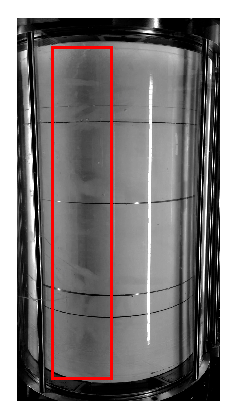
\includegraphics[width=0.4 \textwidth]{Figures/fig4}
%\includegraphics[width=0.9\textwidth]{./graphs/silivery_glow_and_coverage_marked}
\caption{Digitally enhanced photograph of the inner cylinder, covered with the {hydrophobic} coating and visible through the transparent outer cylinder. Estimated is that \SI{99}{\percent} of the inner cylinder is covered by the {hydrophobic} coating. The silvery reflection that is typically associated with the presence of an air plastron, is visible as a darker shaded region. This plastron can only be observed under certain angles of incident light. The curved surface of the inner cylinder explains why the plastron is only visible in a narrow vertical band.}\label{fig:photo_coating_glow}
\end{figure}

\subsubsection{Velocity profile measurements}
Particle Image Velocimetry (PIV) was used to obtain local flow field information. We measured the velocity field in the $(r,\theta)$ plane; $u_\theta = u_\theta (r,\theta,t)$ and $u_r = u_r (r,\theta,t)$. This can only be achieved for single-phase flow with $\alpha = 0$, since the air bubbles otherwise scatter the light significantly. The laser light sheet (Quantel Evergreen 145 laser, \SI{532}{\nm}) used to illuminate the seeding particles added to the flow (Dantec fluorescent polyamide, with a distribution of diameters $\leq \SI{20}{\um}$) was placed at mid-height of the cylinder. Images were captured using a LaVision sCMOS ($2560\times2160$ pixel) camera through the window in the bottom plate of the setup. Figure~\ref{fig:T3C} gives a schematic overview of the measurement setup. Average velocity fields were calculated from 1000 image pairs using LaVision DaVis software in a multi-pass method, starting at a window size of $64\times64$ pixel decreasing to a final size of $24\times24$ pixel with \SI{50}{\percent} overlap.
A calibration is required to transform pixels to meters. To this end image analysis is used to locate the edges of the inner and outer cylinder. Since the measured fields are in Cartesian coordinates, a coordinate transformation is necessary to obtain finally the radial and azimuthal velocities $u_r$ and $u_\theta$ in the cylindrical coordinate system.
